\documentclass[12pt, oneside]{book}   	% use "amsart" instead of "article" for AMSLaTeX format

\usepackage{geometry}                		% See geometry.pdf to learn the layout options. There are lots.
\geometry{letterpaper}                   		% ... or a4paper or a5paper or ... 
\usepackage{parskip}    				% Activate to begin paragraphs with an empty line rather than an indent
\setlength{\parindent}{15pt}
\usepackage{graphicx}				% Use pdf, png, jpg, or eps with pdflatex; use eps in DVI mode
\usepackage{setspace}				% TeX will automatically convert eps --> pdf in pdflatex		
\usepackage{amssymb}
\usepackage{color}
\usepackage{xcolor}
\usepackage{listings}
\usepackage{caption}

\DeclareCaptionFont{white}{\color{white}}
\DeclareCaptionFormat{listing}{%
  \parbox{\textwidth}{\colorbox{gray}{\parbox{\textwidth}{#1#2#3}}\vskip-4pt}}
\captionsetup[lstlisting]{format=listing,labelfont=white,textfont=white,}
\lstset{frame=lrb,xleftmargin=\fboxsep,xrightmargin=-\fboxsep,breaklines=true,basicstyle=\ttfamily\footnotesize}
\lstloadlanguages{ Java, Python}

\begin{document}

\title{\Huge \bf Module Based Development On Android}

\author{A thesis submitted for the degree of\\
Bachelor of Science \\ \\  
by \\ \\ 
Sotaya Yakubu Musa \\ \\ \\ \\ 
Supervised by: \\
Dr. Attila Adamko \\ \\ \\ \\ 
University of Debrecen \\
Center of Arts, Humanities and Science\\
Faculty of Informatics}

\date{2013/2014 Fall Semester}							% Activate to display a given date or no date

\maketitle


\chapter*{\centering STATEMENT}

{\bf ON CONFORMING TO THE RULES OF MAKING A THESIS} \\
I, the undersigned SOTAYA YAKUBU MUSA (Neptun code: AOTNRA) by signing the present statement declare that the thesis entitled 

MODULE BASED DEVELOPMENT ON ANDROID
 
(hereinafter called thesis) is my independent work. In the course of making the thesis I conformed to the rules of Act No. LXXVI of 1999 on Copyright, and the regulations of the University of Debrecen regarding the principles of making a thesis, particularly in respect of the references and citations.

I declare moreover that, in the course of making the thesis, concerning the independent work I did not mislead my supervisor. 

By signing the present statement I take notice of the fact that the University of Debrecen has the right to deny the acceptance of the thesis and to take disciplinary action against me if it is demonstrably not my intellectual creation or if any infringement of copyright falls under suspicion.

The denial of the acceptance of the thesis and the disciplinary procedure do not affect other legal consequences (Civil Law, Law of Petty Offence, Criminal Law) caused by the infringement of copyright.
Debrecen, 2 of December, 2013.				
\\ \\ \\ \\ \\
\_\_\_\_\_\_\_\_\_\_\_\_\_\_\_\_\_\_\_\_\_\_\\
Student�s signature 

\newpage
\thispagestyle{empty}
\mbox{}

\chapter*{\centering Abstract}
\addcontentsline{toc}{chapter}{Abstract}%
This work represents a detailed study of modular development approach, android platform and the technologies accompanied by them. The motivation for this work is derived from the problem faced with developing complex systems and my love for developing android applications. Modular development is a software development approach that emphasizes on dividing a software system into logically functional units (named modules) that can be assembled into a larger system. The software system developed to show the practical application of this approach is a surveillance system, which can run on android devices with the support for camera's. Users can monitor a particular environment with the software system and whenever a face is detected, the user gets notified via both email and sms. This thesis contains both the modeling and implementation of the system adhering to the modular development approach. 

\begin{doublespace} {\large {\it "It is the way I think. I am a very bottom-up thinker. If you give me the right kind of Tinker Toys, I can imagine the building. The converse is true, too, I think. I can�t from the building imagine the Tinker Toys. When I see a top-down description of a system or language that has infinite libraries described by layers and layers, all I just see is a morass. I can�t get a feel for it. I can�t understand how the pieces fit; I can�t understand something presented to me that�s very complex. Maybe I do what I do because if I built anything more complicated, I couldn�t understand it. I really must break it down into little pieces."} \\ \\ 

Ken Thompson}
\end{doublespace}


\tableofcontents


\cleardoublepage
% \phantomsection
\addcontentsline{toc}{chapter}{\listfigurename}
\listoffigures

\cleardoublepage
% \phantomsection
\addcontentsline{toc}{chapter}{Listings}
\lstlistoflistings

\chapter{Introduction}
{\it A programmer has this intelligent idea to develop a system that will change the world, this system is so big that it might need more than one developer to make it happen, even if the programmer decides to do it alone, he needs to develop it in such a way that he can handle its complexity.}

From the story above, the question "how can one effectively develop a complex software system that is flexible, extensible, manageable and maintainable?" is derived, this is the question I hope to answer in this thesis. 

{\bf Software development} have become a crucial part of our community today, as almost every business, research, 
experimental and educational sector requires software solutions to problems. With this comes a high need to develop
good software systems that not only serve the required functionalities, but also is flexible, extensible and efficient. This 
softwares are developed by {\bf Software Developers}, whom face problems of their own, problems such as good development
processes and methodologies that enables them develop systems efficiently, deliver software products on time, ease in
both development and management, and cope with the ever changing of software requirements.


Through the period of my studies, I have come to discover, attain and apply various set of skills ranging from creativity, research, critical thinking, problem solving, to the whole process involved in software engineering such as; requirements gathering, software design, implementation, testing and management of evolving systems. Though I had lots of challenges during the course of my studies, I have come to develop interest in Application of Artificial Intelligence such as Computer Vision, Intelligent Agents and Robotics, Software development on Desktop, Mobile and Embedded platforms, Modular Systems, programming methods, paradigms and methodologies. 


Mobile market is one of the biggest markets of our time, with more and more mobile platforms being developed. Android have been at the top of the market with over 52 percent of the market and with over 1.5 million android devices activated per day. It is very clear that this is where every developer will want to be. Besides the joy of writing applications that will possibly be used by millions of people, developing solutions to problems faced by developers of this platform happens to be of great interest to me.


I have done some development on Android platform, explored its various features and this lead me to conceptualize various ways i can simplify and develop complex systems. Being a man of structure and simplicity in terms of software development, discovering modular development was a great breakthrough for me, though this method have existed for quite a while now some might view it as old fashion and ineffective. Breaking a complex system into smaller chunks (modules) based on functionalities and developing each module independently with little or no connection to others seems so intelligible and exquisite to me.


In the chapters to come, I am going to discourse and explore the concept of modularity in software development, why it is important and how it can be achieved. With the aid of the android software system i developed using both the native development tool Android SDK with Java and Kivy Framework with Python, I will explain and show how this method can be applied. Development using both of this environment was an idea from my supervisor Dr. Attila Adamko, which turns out to be a really good one in terms of making the points of this thesis.


\chapter{Literature}
\section{Modular Development}
When it comes to software development, there are a bunch of approaches and for a fact, no single approach can be labeled as the best but can be the best in terms of a certain kind of system. When developing complex systems, whether in teams or as an individual, sometimes one tends to lose perspective when development becomes really bogus and in turn causes a project failure either due to the inability to produce the product that meets the customers requirements or due to complexity causing the management  of the software to be tedious. The idea of Modular Development is to overcome this problem of complexity by designing and developing a system that is manageable, simple and comprehensible simply by dividing the whole system into smaller units that can be managed individually. 

Modularity is a bit redundant as there are lots of different definitions of what a module really is, most of the definitions out there have no experimental proof. The word module is an overloaded term and can mean a number of things, in this thesis, the word module means an independent functional unit of an application that has no or less dependency on other modules except in point when it need another module to achieve it purpose. In this sense, a module will be represented either as a package or an application that can easily be removed or integrated into a bigger system.

Modular development or sometimes known as Modular approach to Software Development is a development technique that covers from the design to the implementation of software systems in terms of components or modules. This idea focuses on the separation of concerns, in which each functionality is developed as a module which is a logically discrete function and has no or less communication with other modules, except the point whereby it requires another module to achieve its purpose. 

Modular development consists of {\bf modular programming} which in turn has two aspects, being, design and implementation. These involves the software design technique and the implementation of the working code based on that design respectively. 

\subsection{Modular Programming}
{\bf Design}\\
{\bf Modular design} concentrates on the architectural design of a software system in terms of modules, in this design, the modules have to be clearly represented in such a way that each describes a logically discrete function and is comprehensible at first glance. The design tends to show the system modules as independent, scalable and reusable components and also the ease in extending the system with the matter of plugging new modules to it. 

It is important to design a modular architecture of a software system first before its implementation showing all dependencies, in this case, it will be difficult for the system to degenerate into an unmaintainable system without being noticed during development. There are a lot of tools that can be used to design a software systems architecture including UML tools, tools like Visual Paradigm for UML, UMLet, Rational Rhapsody e.t.c

\noindent {\bf Implementation}\\
This phase involves the {\bf implementation} of a software system by the aid of a modular architecture of the system and a programming language that supports or aids modularity. This method of programming disallows the use of control variables and flags which enables the caller to successfully call a module without knowing the details of how it was implemented. 

{\bf Modular programming} encourages the separation of concerns, dividing a system into independent modules such that each module performs a logically discrete function. There are different levels to which modularity can be achieved (depending on the size and type of the system); 1) Application level 2) Package level 3) Function/Method level. Programming languages that support modularity allows us to comfortably divide our system independently into the above stated levels. Specifically, in this thesis with the aid of our project, we will see how a system can be developed using the modular approach i.e dividing the system into package level modules and application level module receptively.

There are lots of languages that support modular programming, such languages are; C/C++, Java, Python, Perl, Pascal, Algo e.t.c.  And some of this programming languages provide us the feature of module encapsulation. Encapsulation is a method of hiding (in our case) module information from other modules, in other words, modules that do not have dependencies on others cannot access their information. This feature especially makes it possible to control module interdependencies and flexibility when managing and maintaining system modules, also allows us to avoid developing a monolithic bunch of tightly coupled code.

In modular programming, modules can communicate or be used by a system by {\bf Message} passing or the more conventional {\bf Call}. When a module is being called, control is handed over to that module and it will be so until the module is done with its operation there by handing control back to the caller. However, in some technologies now, it is possible to run multiple tasks at the same time by the use of "Threads".

\section{Benefits of applying Modular Development}
I have talked about modular development to a certain degree of detail, explaining how the structure is and different processes involved in this particular approach to software development. However there are a number of advantages of applying this technique to software development and some of those are: 
\begin{itemize}
\item{\bf Structured approach,} complex problems or systems can be broken down into smaller and simpler tasks that can be managed easily and maintained with less stress. This kind of approach sometimes referred to as the top-down design, which means, when there is a problem, it is split into smaller units and those units are in turn split into much smaller ones until the lowest functional level is reached.
\item{\bf Separation of concerns,} with this approach, we can easily separate different aspects of a system into modules in such a way that each (module) deals with a single logically discrete function with no interaction with other modules unless it needs another module to achieve its goal and one can easily look at a module and describe what it does in a single sentence. 
\item{\bf Distributed development,} modular development allows distributed development. By breaking down a complex system into smaller modules, each of this module can be assigned to be developed by a separate team or individuals, sometimes located in a different geographic region without any inconvenience. As one of the goals of this technique is to be able to utilize a module without having any idea on how it was developed, each modules can then be assembled or integrated into a system by someone other than their developers with less or no knowledge of how it was implemented.
\item{\bf Reuse,} by dividing a system into modules, a module can be reused throughout a system, this reduces code redundancy. Also not only can it (the module) be used in the same system it was developed for, but also can be utilized in projects in the future when a certain functionality it gives is needed.   
\end{itemize} 


\chapter{Development Platform}
This thesis is accompanied by a project developed to present a proof of the concept discussed in the previous chapter as just stating or realizing the concept itself is not enough. The project is based on the modular approach to software development on {\bf android} platform. It is however very important to introduce this platform properly, stating the different technologies available and its structure to give a general idea of what this project is developed on (though this chapter will not teach android development but merely give an introduction to the platform). 

In this chapter, i will be introducing the android platform itself, structure of the android virtual machine (AVM), development environment including the integrated development environment (IDE) used, the software development kit (SDK), android virtual device (AVD) and Kivy framework which was used to develop one of the modules of these thesis project. 

\section{Android}
Android is an Open Source Linux-based mobile operating system which was first developed by Android Inc. and later acquired by Google Inc. Google market the android platform to handset makers providing them with constant software upgrades and features, this platform grew gradually and became the first product of the open standards developed by the open handset alliance which includes companies such as HTC, Sony, T-mobile, Samsung, Qualcom, Sprint Nextel, Texas Instrument and Google.

The openness of android is worth mentioning, as Google releases the software source code under the Apache License, this makes it possible for manufacturers to modify, customize and distribute the software freely. 

With the large community of android developers, developers are constantly developing applications and tools that extends the functionalities of the software, making it one of the most popular and supported mobile platform of this age. Development of android applications is done with the customized version of Java programming language, however, over the years other frameworks and SDK's such as Kivy, Cordova, Corona e.t.c have been developed which makes it possible to to write android apps with other languages such as Python, C sharp and web technologies (HTML, CSS and JavaScript).

Android being the most widely used mobile operating system, users have access to more than 800,000 applications in the Google Play Store in which over 700,000 of those are free.
 
\section{Android Architecture}
The Android operating system contains a stack of software components which are divided into four layers, each layer contains in turn important program components and renders various services to the layer immediately above it. Description of each layer (from bottom up) as shown in the android architecture diagram (Fig 3.1). 

\begin{figure}[ht!]
\centering
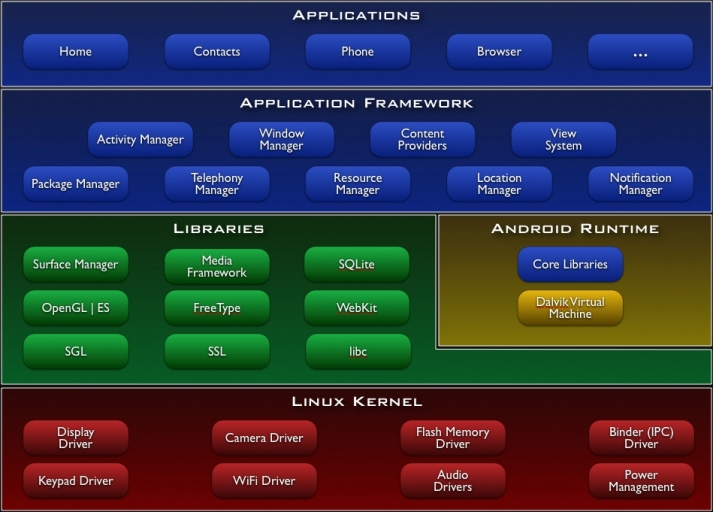
\includegraphics[width=150mm]{android_architecture.jpg}
\caption{Android architectural diagram }
\label{overflow}
\end{figure}

 \begin{itemize}

\item{\bf Linux kernel}
 At the lowest level is the Linux kernel in which the whole android OS was built on. Linux kernel contains various hardware drivers and communicates directly with the device hardware. It provides some services such as the hardware management, memory management, networking, process management e.t.c
 
 \item{\bf Libraries}
 The layer on top of the Linux kernel is the android native libraries containing a set of libraries which are written in C/C++ and provides the device the capability of handling different types of data. Some of this libraries include surface manager, media framework, SQLite, OpenGL, WebKit, SSL, libc e.t.c This libraries are called through Java interface and used to store data, seek hardware service such as the camera, internet security e.t.c
 
\item{\bf Android Runtime}
 This layer of the architecture contains the Dalvik Virtual Machine which is a customized Java Virtual Machine designed and optimized for android, it is developed to suit the needs of systems that are constraind in terms of processor speed and memory. It runs the android applications each in its separate process, by utilizing the Linux features such as the memory management and multithreading. The Android runtime also contains Java core libraries enabling developers to write android applications using the Java programming language. Android programs written in Java are compiled to bytecode, after which they are converted from Java Virtual Machine compatible .class to Dalvik compatible .dex which is the dalvik executable. 
 
 \item{\bf Application Framework}
 This block provides high level services that enable application developers to use directly in their application. This services are provided as a form of Java classes, and are used to manage basic functions such are the views, activities, notifications e.t.c
 
 \item{\bf Applications}
 This layer is where all the applications reside including some built-in applications that comes with the OS, applications such as the Web Browser, Contact Manager, Games, Dialer e.t.c 
 
\end{itemize}

\section{The Development Environment}
For developers to be able to write android application, they will need some development tools. This development tools provide a programming interface for the developers to easily write applications using the Java programming language.

\subsection{Android SDK}
The software development kit provides a comprehensive set of development tools, it contains packages, application framework, libraries, debugger, documentation, emulator, sample codes and other tools that are used in the development of android applications. 

\subsection{Android Virtual Device}
The android virtual device manager helps developers to emulate different android mobile phones. As there are a lot of different android phones out there with various screen resolutions, it is important for developers to be able to test their application on different types of devices, android virtual device manager solves the problem of not needing to own different android devices in other to test applications. 

\subsection{Eclipse IDE}
Though Eclipse Integrated Development Environment is not mandatory for android developers, it have been recommended to be used. Eclipse have been the official IDE for android development as it makes it easier, faster and straight forward to develop applications once one have setup the environment properly. 

\section{Kivy}
As stated earlier, the project presented in this thesis was developed using both android native development platform and the kivy framework. The idea was to develop a module completely in a different language, showing the flexibility of modular development. As the framework uses Python programming language as its back-end language, there are a lot of awesome features of Python that are worth mentioning.

Python is a general-purpose, dynamic, high-level and multi-paradigm language which is widely in use, and its structure focuses on code readability which can be seen from the enforced code indentation as part of its syntax. Python being an interpreted language, can be used as both a full fledged language and can be integrate together with another language as a scripting language.

However, the aspect of Python that is most attractive especially to this thesis is its high support for modularity. This feature have been transferred to the Kivy framework and there is a clear separation of concern between the user interface and the back-end Python code. Another feature of Python that makes it attractive is the ease which features can be implemented fast and with less lines of codes compared to other languages.   

Kivy is an open source Python library developed by the Kivy organization alongside Python for Android. It is a framework for rapid application development of multitouch applications with natural user interface (NUI), which is distributed under the MIT license.

Kivy framework contains all that is needed to develop an application. Having components such as the support for mouse, keyboards, widgets that support multitouch, the Kv language in which is used to design the user interface. Application developed with Kivy can be run on multiple platforms (Linux, Windows, Android, IOS) with the aid of the Kivy Launcher which is available for all the platforms, or can be compiled as an executable for the desired platform. 

\begin{figure}[ht!]
\centering
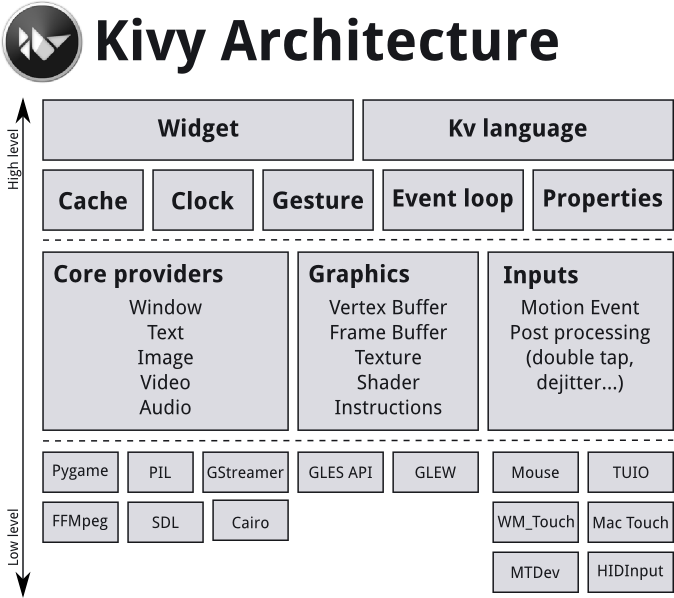
\includegraphics[width=120mm]{kivy_architecture.png}
\caption{Architectural diagram of the Kivy Framework}
\label{overflow}
\end{figure}



\chapter{Project Overview}
In order to present a practical solution and application of the discussed modular development approach to development of complex software systems, a project have been developed to support the theory and show the way it can be achieved. Some aspects of the implementation have been left out for the reason of being trivial and basic when it comes to android development, areas such as layout design, environment configuration, values and drawable settings, this aspects are unique from developer to developer and can be set as pleased. Though some important pointers will be stated where deemed.

This project is a surveillance application which i named "Eye Droid". The idea behind it is to develop an Android application that will make use of an android device camera to monitor a particular surrounding, notifying the user in real time, whenever a face is detected. This is a great idea considering there are lots of android devices out there ranging from mobile phones, native cameras, tablets and other embedded devices.

The project will cover the structure of the system, the system models showing different perspectives of the system including use case diagram,  class diagram and show the screen shot of each activity. Also the implementation of the individual module that constitutes this software system will be discussed in detail along side the code snippets. 

\section{System Structure}
The architectural representation of this system shows the high-level structures of the software system. The structure of how the modules fit into the system is shown by the architectural diagram of the system followed by the brief description of each module.

\begin{figure}[ht!]
\centering
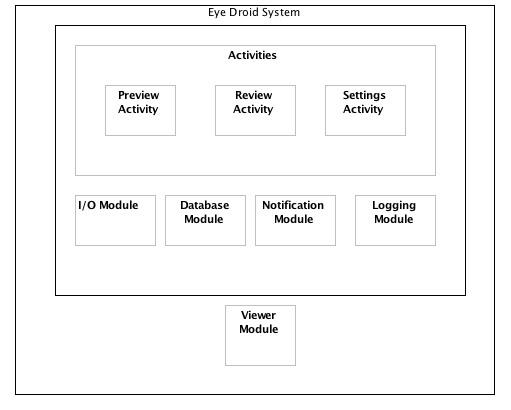
\includegraphics[width=140mm]{eye_arch.png}
\caption{Eye Droid System Architecture}
\label{overflow}
\end{figure}    

Modules present in this system as shown in listing 4.1 are the {\it I/O module, database module, notification module, logging module and viewer module}. The modules a structured in terms of packages (as the Java programming language provides us the means to modularize using this feature) except for the viewer module which is an application level module, and its installed separately in the system then called through the use of {\bf intents}. Apart from the modules implementation of the application, activities are also discussed. 

\begin{itemize}
\item {\bf I/O module}, this module contains a set of methods defined to handle different types of input and output operations. This module is used by the system Activities and also by some modules as they require some I/O operations.

\item{\bf Database module}, this module is responsible for the SQLite database connection, reads and writes. It is also used by the notification module to log some certain events that happened during the camera preview.

\item{\bf Notification module}, this modules deals with the EMAIL connection, sending of messages and attachments when it is called. This module is used by the Preview activity when notifying the user when a face is detected and also by the review activity when uploading the log file generated from the database.
 
\item{\bf Logging module}, this module is an android service, it is automatically started when the preview activity is started and it runs in the background listening to some certain events and logging them into the SQLite database using the database module.

\item{\bf Viewer module}, this module is an application level module developed using the Kivy framework, it is a simple image viewer module that displays images of faces detected and provide small features like enlarging, shrinking and rotation. It is called by the Main activity through intents.
\end{itemize}
The application also contains user settings informations, information such as email, password, phone number e.t.c This information are stored in the user preferences, which is a file that exist in the system and can be read or written into very easily.

\section{Activities}
Activities are the presentation layer of an Android application, an application consist of one or more activities and an activity can pass data or control to another activity by the use of the interprocess communication protocol called {\bf intents}. Each activity consist of a single visual user interface (that is what the user sees with the buttons and images e.t.c) designed using XML and accompanied by a java class which contains the code responsible for handling the various types of widgets in the GUI. In this thesis i will not discuss the graphical representation of an activity as it is basics and anyone can get a hang of it, however i will discuss the back-end code responsible for handling this views.

Each activity has a structure and a set of events that can be implemented to control the lifecycle of the activity. Each event is a method that is called depending on what phase the activity is in the lifecycle.

\begin{figure}[ht!]
\centering
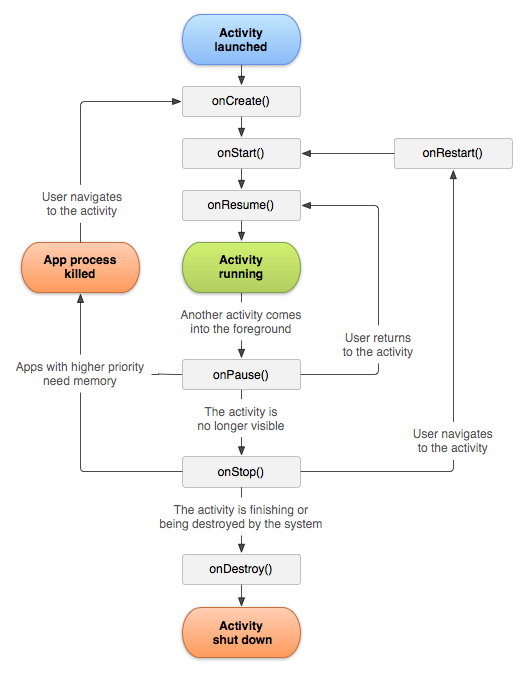
\includegraphics[width=110mm]{activity_lifecycle.png}
\caption{Android Activity lifecycle}
\label{overflow}
\end{figure}

\begin{itemize}
\item{\bf onCreate()} This is called when the activity is started, and to perform a one-time initialization of objects instances leading to the launch of the individual interface. It contains a parameter that has information gotten from the {\it onSaveInstanceState()} method which is the previous state of the activity and can be null if there was no previously saved state.
\item{\bf onStart()} This is called after the {\it onCreate()} method have complete initialization and content is ready to be shown to the user.
\item{\bf onResume()} This is called when the activity is to be brought to the foreground and ready to continue from where it was left off.
\item{\bf onRestart()} This event is triggered after an activity have been stopped (not paused) and started again. Which in other words the activity is redisplayed to the user.
\item{\bf onPause()} this is triggered when another activity is brought to the foreground, either by the user when navigating to another activity of because another application with higher priority needs memory.
\item{\bf onStop()} This is called when the activity is no longer visible. If there is need for memory, this event can also be triggered by the OS.
\item{\bf onDestroy()} This is called just before the activity is destroyed, either by the user finishing the activity or by the system when it needs memory.
\end{itemize}

The following are the list of activities present in the {\bf Eye Droid} project:
\begin{itemize}
\item{\bf Main activity}, as the name implies, this is the first screen a user will see after the splash screen. It contains various image buttons that leads to different activities. The preview button, review button, settings button and viewer button.
\item{\bf Preview Activity}, this is the activity that captures the camera preview, and detects faces, it displays the preview alongside the number of face label and the capture button.
\item{\bf Review Activity}, simply displays the log content to the user, and provides option to either wipe clean the log or upload the log.
\item{\bf Settings Activity}, this activity provides an interface for the user to set email, password, phone number e.t.c and save to the user preferences. 
\end{itemize} 

\section{Intent}
{\bf Intent} is an abstract description of an operation to be performed, it allows application components to request functionalities from other android components. {\it startActivity} can be used to launch an activity and {\it startService(Intent)} to start and communicate with a background service.

An intent structure contains 6 parts:
\begin{itemize}
\item {\bf action}, the action to be performed e.g "ACTION\_VIEW", "ACTION\_DIAL"
\item {\bf data}, the data to be acted upon
\item {\bf category}, information on the action to be executed
\item {\bf type}, explicitly specifies the type of intent data
\item {\bf component}, explicitly specifies the name of the component to be used by the intent
\item {\bf extras}, a Bundle which contains additional information for the component.
\end{itemize}


\chapter{Project Modeling}
As discussed in chapter 2 of this thesis, modular development requires a description and design of the system before implementation, this descriptions and designs will ensure that the software system being developed meets the needs of the user or customers and to serve as a guideline throughout the development process. 

Implementation on the other hand will be much more less tedious and straight forward in the presence of a pre-development design. Not only in this approach, it is always important to design once system before it is implemented. Various Software development models adhere to this standard. The previous chapter shows a brief explanation with diagram of the structural representation of this system, this chapter on the other hand will solely deal with the description models.

Purpose of a software model is to reduce the ambiguity of a software requirement descriptions which is mostly in natural-language and provide a visualization of a system design which in turn can be debated on. Models also show the system to be developed from various perspectives. This project will be modeled using two of the UML diagrams, as such, it is important to talk about the basics of UML and its diagrams in order to comprehend this modeling.

\section{UML Diagrams}
Unified Modeling Language (UML) is a general purpose modeling language which is used in software engineering field to model software systems. The Unified Modeling Language was developed in the 1990's by {\it Ivar Jacobson, James Rumbaugh and Grady Booch}. In 1997 Object Management Group (OMG) adopted this project and they have been managing it ever since.

Unified Modeling Language being the industry's standard for modeling object-oriented software-intensive systems (accepted in 2000 by the International Organization for Standardization) contains various set of graphical notations that are used to visualize system models. There have been various versions of the evolving UML throughout the years, with each version denoted e.g UML 1.x, however, the current version was released August 2011 being the UML 2.4.1. 

There are fourteen UML diagrams that are used to model software systems as of the UML version 2.x, this diagrams are divided into structural and behavioral diagrams. Under behavioral diagrams there is the interaction diagrams.

{\bf Structure Diagrams:}
\begin{itemize}
\item{Class Diagram}
\item{Object Diagram}
\item{Package Diagram}
\item{Component Diagram}
\item{Composite Structure Diagram}
\item{Deployment Diagram} and, 
\item{Profile Diagram}
\end{itemize}

{\bf Behavior Diagrams:}
\begin{itemize}
\item{Use Case Diagram}
\item{Activity Diagram}
\item{State Machine Diagram}
\item{\bf Interaction Diagram:}
\begin{itemize}
\item{Sequence Diagram}
\item{Communication Diagram}
\item{Interaction Overview Diagram}
\item{Timing Diagram}
\end{itemize}
\end{itemize}

\section{Use Case Diagram}
A {\bf use case diagram} in its simplest shows the interactions between a system and its various user's, depicting the specification of a use case. Use case diagram can show the different types of user's and the different ways they interact with the system individually. The diagram is in conjunction with a use case and other supporting diagrams. A simple illustration of a use case diagram is presented in Figure 5.1.

\begin{figure}[ht!]
\centering
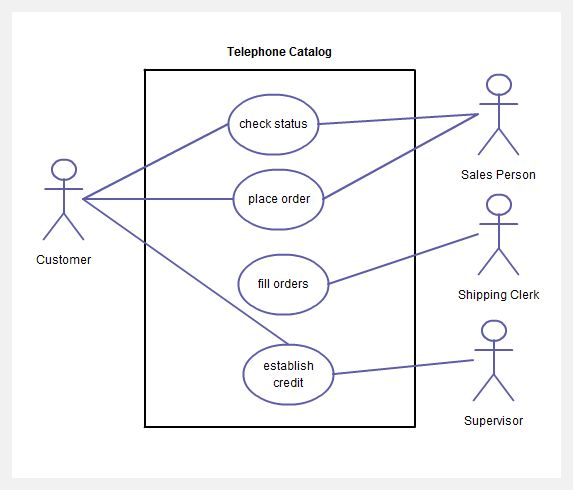
\includegraphics[width=110mm]{usecase_diagram.png}
\caption{A simple Use Case Diagram}
\label{overflow}
\end{figure}

A use case diagram can say a thousand words to the developer, as not only does the developer have the specifications but also sees visually how the user is going interact with the system. This solves the problem of developers wandering away from the main objective of a system. Also users of the system will prefer a visual depiction of all the possible use cases and can give them a general idea of the operations involved in the system.
\newpage
\subsection{Eye Droid Use Case Diagram}

\begin{figure}[ht!]
\centering
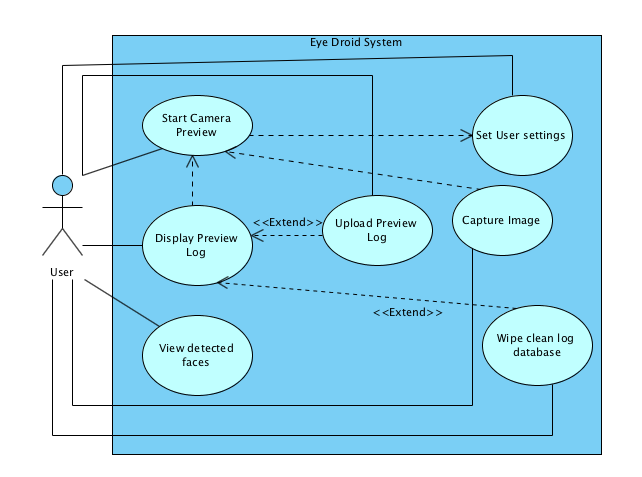
\includegraphics[width=150mm]{eye_droid_usecase_diagram.png}
\caption{Eye Droid Use Case Diagram}
\label{overflow}
\end{figure}   

\section{Class Diagram}
A {\bf class diagram} is a structured diagram that describes the structure of a system by showing the system's classes, their attributes, operations (or methods), and the relationships among objects. Class diagram is the main building block of object-oriented modeling, and since our platform's native programming language is Java, it is important to provide this diagram.

\begin{figure}[ht!]
\centering
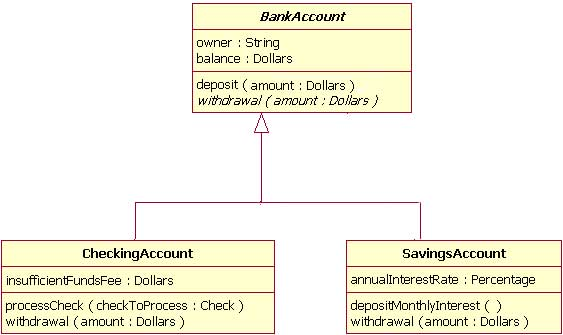
\includegraphics[width=140mm]{class_diagram.jpg}
\caption{A Simple Class Diagram}
\label{overflow}
\end{figure}   

Figure 5.3 shows a simple class diagram of the classes {\it BankAccount, CheckingAccount and SavingsAccount}. It gives a detailed description of the classes and their relationships.

\begin{itemize}
\item{\bf BankAccount Class}, this class from the figure shows a bank account which has the fields "owner" which is a string, "balance" which is in dollars and two methods "deposit" and "withdrawal" - both taking a parameter amount in dollars.
\item{\bf CheckingAccount Class}, this class contains the fields "insufficientFundsFee" which is in dollars and two methods that allows withdrawal and process check.
\item{\bf SavingsAccount Class}, this class contains a field "annualInterestRate" which is a percentage of the annual interest  and two methods for checking monthly deposit interest and withdrawal.
\end{itemize}

From this classes, it is clearly seen that both {\it CheckinAccount and SavingsAccount class} extend the {\it BankAccount class} and in turn inheriting and implementing one of its methods, "withdrawal."
\newpage
\subsection{Eye Droid Class Diagram}  

\begin{figure}[ht!]
\centering
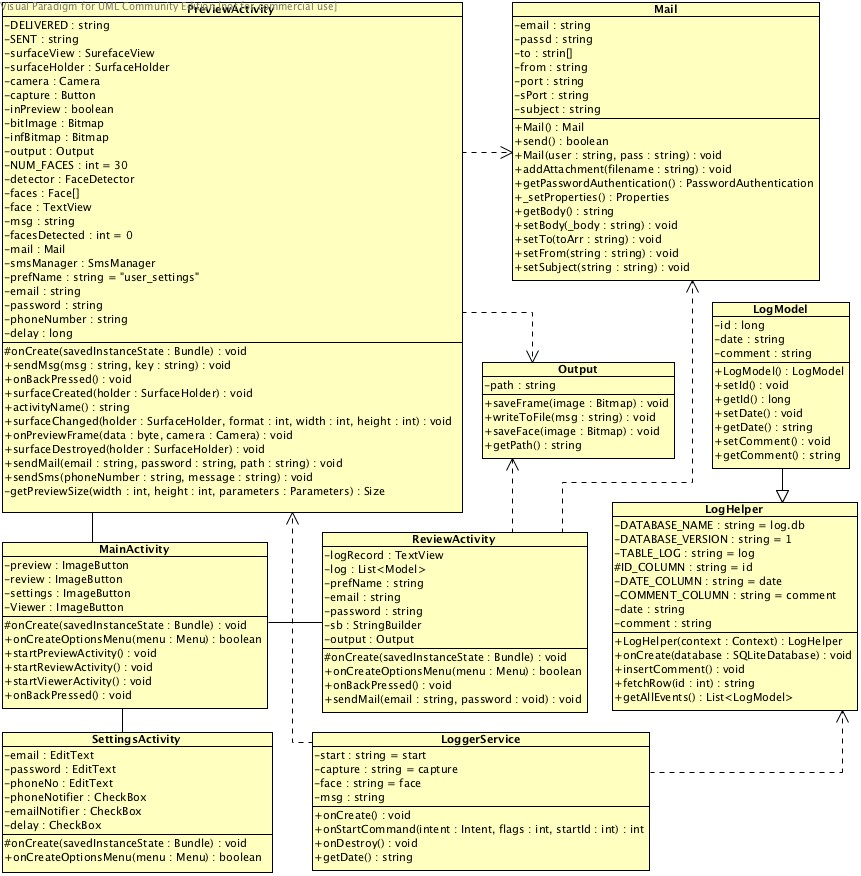
\includegraphics[width=170mm]{eye_droid_class_diagram1.jpg}
\caption{Eye Droid Class Diagram}
\label{overflow}
\end{figure}   


\chapter{Implementation}
When talking about software development processes, there is always an implementation phase which is the stage that the actual coding takes place, in respect to the earlier design phase. Modular development is not an exception, this stage of modular development is the so called {\bf modular programming} and this stage will make use of the modelings made in the previous chapter to implement the {\bf eye droid} system.

In this chapter, only the core part of the system will be discussed, code listings will be provided to show how this system was implemented. Since this development was done for the android platform using the native android language and Kivy framework, Java programming language will mostly be used and in a later module Python programming language.

Modular development approach is the target approach for developing this software system, as such, the package feature of the java language was used to divide the application into modules and also with one module which is an application level module.

\section{I/O Module}
The {\bf input and output module} is a package which consists of a single class {output.java} this module handles all the I/O operations that is needed in this particular software. Within the class, three methods have been developed to handle saving files on the device's local storage, files such as images (.jpeg, .png e.t.c) and text files. The three methods include ({\it saveFrame(Bitmap), writeToFile(String), saveFace(Bitmap)}) all this methods contain the same structure and differ only by storage destinations and type of files, in which case, one method is sufficient to understand this module. 

\begin{lstlisting}[label=Saving-a-file-in-device-storage-drive,caption=Saving files in device storage drive]
public void saveFace(Bitmap image) {
	try {
		String root = Environment.getExternalStorageDirectory().toString();
		File dir = new File(root + "/org.plaix.viewer/Images");
		dir.mkdirs();
		Date date = new Date();
		CharSequence sequence = DateFormat.format("MM-dd-yy-h-mm-ss",
				date.getTime());
		String imageName = "Image-" + sequence + ".jpg";
		path = root +"/org.plaix.viewer/Images/"+imageName;
		File file = new File(dir, imageName);
		FileOutputStream fos;
		fos = new FileOutputStream(file);
		image.compress(Bitmap.CompressFormat.JPEG, 90, fos);
		fos.close();
	} catch (FileNotFoundException e) {
		e.printStackTrace();
	} catch (IOException e) {
		e.printStackTrace();
	}

}
\end{lstlisting}

Listing 6.1 shows the method {\it saveFace()} which takes a single parameter of type {\it Bitmap}, gets the path to the devices's local storage with the method {\it Environment.getExternalStorageDirectory()}, creates a file(directory) and concatenate the root directory with the directory in which the file is to be saved to. After creating the file, a name for the file is generated, a {\it FileOutputStream} object is created with the file and the image is compressed into a JPG format using the method {\it Bitmap.compress()} with parameters of the format and the file output stream.

\newpage
\section{Database Module}
The {\bf database module} contains two java classes, one is an implementation of the relational model of the database (LogModel.java) describing the structure of the database. The second class (LogHelper.java) is the implementation of the {\it SQLiteOpenHelper} which is a helper class to manage the creation, opening, upgrading and versioning of the database.  

\begin{lstlisting}[label=database-relational-model,caption=Relational Model of the Database Module]
public class LogModel {
	private long id;
	private String date;
	private String comment;
	
	public LogModel(){}
	
	public LogModel(long id, String date, String comment){
		this.id = id;
		this.date = date;
		this.comment = comment;		
	}
	
	...
	
	@Override
	public String toString(){
		return id+". "+date+": "+comment;
	}
	
}
\end{lstlisting}

From the code listing above (listing 6.2) it is easy to deduce the structure of the database having a single table with the columns {\it id, date and comment}, also having two constructors for instantiating the model object, one taking no arguments and the other taking three arguments each being a column in the table. This is also accompanied by a set of {\it getters and setters}. The {\it toString()} method was overridden to return the columns in the desired format as shown in the listing.
\newpage
\begin{lstlisting}[label=sqlite-helper,caption=Implementaion of the SQLiteOpenHelper] 
	...
	
	public LogHelper(Context context, String date, String comment){
		super(context, DATABASE_NAME, null, DATABASE_VERSION);
		this.date = date;
		this.comment = comment;
	}
	
	public LogHelper(Context context){
		super(context, DATABASE_NAME, null, DATABASE_VERSION);
	}
	
	@Override
	public void onCreate(SQLiteDatabase database) {
		database.execSQL(CREATE_DATABASE);
	}

	@Override
	public void onUpgrade(SQLiteDatabase database, int oldVer, int newVer) {
		database.execSQL("DROP TABLE IF EXISTS " + TABLE_LOG);
		onCreate(database);
	}
	
	public void insertComment(){
		SQLiteDatabase db = this.getWritableDatabase();
		ContentValues values = new ContentValues();
		values.put(DATE_COLUMN, date);
		values.put(COMMENT_COLUMN, comment);
		db.insert(TABLE_LOG, null, values);
		db.close();
	}
	
	public List<LogModel> getAllEvents() {
	    List<LogModel> logList = new ArrayList<LogModel>();

	    String selectQuery = "SELECT  * FROM " + TABLE_LOG;
	 
	    SQLiteDatabase db = this.getWritableDatabase();
	    Cursor cursor = db.rawQuery(selectQuery, null);
	 
	    if (cursor.moveToFirst()) {
	        do {
	            LogModel log = new LogModel();
	            log.setId(Integer.parseInt(cursor.getString(0)));
	            log.setDate(cursor.getString(1));
	            log.setComment(cursor.getString(2));
	            logList.add(log);
	        } while (cursor.moveToNext());
	    }
	    db.close();
	    return logList;
	}
	
	public void cleanDB(){
		SQLiteDatabase db = this.getWritableDatabase();
		db.delete(TABLE_LOG, null, null);
		db.close();
	}
\end{lstlisting}

In the second class of this module, seven important methods are to be discussed as shown in listing 6.3. 
The first two methods {\it LogHelper(Context, String, String), LogHelper(Context)} are constructors for instantiating the object of this class. They both contain argument "Context" which is an interface to global information about an application environment provided by the android system. 

The third method is the {\it onCreate()} method which has an initial implementation in the super class {\it SQLiteOpenHelper} and needs to be overridden and implemented, this method as the name implied is used to create tables and initially populate them by executing the SQL statement "CREATE\_DATABASE". The method is called whenever the database is created for the first time.

The {\it onUpgrade()} method like the {\it onCreate()} need also to be reimplemented. This method is called whenever the database needs to be upgraded, it has to first drop the existing tables and call the {\it onCreate()} method to recreate the database and upgrade the new schema version.  

The final set of methods are the {\it insertComment(), getAllEvents(), and cleanDB()}. The {\it insertComment()} simply creates a new SQLite database object using the {\it getWriteableDatabase()} method, creates a new ContentValues object and set the values of each of the "date" and "comment" column then writes it to the database using {\it SQLiteDatabase.insert()} method.
{\it  getAllEvents()} method on the other hand executes a select statement on the existing database, storing the result in a cursor structure which makes it easier to iterate through the elements and set the respective values to the {\it LogModel} object instance returning all the results in a list. The final method of this helper class is the {\it cleanDB()} method which simply truncates the desired database table. 

\section{Notifier Module}
The {\bf notifier module} is responsible for handling all types of notification systems, the major notification systems used in this project are the Email and Sms notification systems. Within this module, there is a single class which extends the {\it javax.mail.Authenticator} class (Java mail api) and consists of several methods for configuring authentication, message body and attachment. This module was developed in such a way that when sending email, the android smtp client not need to be started, instead everything it is configured internally and mail is sent automatically. 

\begin{lstlisting}[label=Mail-constructor,caption=Java Mail Api Constructor] 
public Mail() { 
    port = "465";
    sPort = "465"; 

    email = "";
    passd = ""; 
    from = ""; 
    subject = "";  
    body = ""; 
    debugable = false;  

    multipart = new MimeMultipart(); 
    
    ...
    
  }
\end{lstlisting}

The java mail api constructor shown in listing 6.4 sets the smtp's, default socket, factory ports, email, password and other required parts of an email such as from, to, subject and email body which are all initially empty. Later the constructor instantiates the multipart object, this object configures the email body in such a way that when it is too long, it splits it into multiple parts.
\newpage
\begin{lstlisting}[label=Mail-send,caption=Send Method] 
public boolean send() throws Exception { 
    Properties props = _setProperties(); 

    if(!email.equals("") && !passd.equals("") && to.length > 0 && !from.equals("") && !subject.equals("") && !body.equals("")) { 
      Session session = Session.getInstance(props, this); 

      MimeMessage msg = new MimeMessage(session); 

      msg.setFrom(new InternetAddress(from)); 

      InternetAddress[] addressTo = new InternetAddress[to.length]; 
      for (int i = 0; i < to.length; i++) { 
        addressTo[i] = new InternetAddress(to[i]); 
      } 
        msg.setRecipients(MimeMessage.RecipientType.TO, addressTo); 

      msg.setSubject(subject); 
      msg.setSentDate(new Date()); 

      BodyPart messageBodyPart = new MimeBodyPart(); 
      messageBodyPart.setText(body); 
      multipart.addBodyPart(messageBodyPart); 

      msg.setContent(multipart); 
      Transport.send(msg); 

      return true; 
    } else { 
      return false; 
    } 
  }
\end{lstlisting}

The code snippet in listing 6.5 shows the {\it send()} method, this method when called creates a new session using the properties provided by the {\it \_setProperties()} method. With the session, a MimeMessage object is created and sent after its fields (i.e from, to , subject e.t.c) have been set

\begin{lstlisting}[label=Mail-send,caption=Mail configuration] 
public void addAttachment(String filename) throws Exception { 
    BodyPart messageBodyPart = new MimeBodyPart(); 
    DataSource source = new FileDataSource(filename); 
    messageBodyPart.setDataHandler(new DataHandler(source)); 
    messageBodyPart.setFileName(filename); 

    multipart.addBodyPart(messageBodyPart); 
  } 
 
  @Override 
  public PasswordAuthentication getPasswordAuthentication() { 
    return new PasswordAuthentication(email, passd); 
  } 

  private Properties _setProperties() { 
    Properties props = new Properties(); 
    
    if(debugable) { 
      props.put("mail.debug", "true"); 
    } 
    /*
    if(_auth) { 
      props.put("mail.smtp.auth", "true"); 
    } */
    props.put("mail.smtp.auth", "true");
	props.put("mail.smtp.starttls.enable", "true");
	props.put("mail.smtp.host", "smtp.gmail.com");
	props.put("mail.smtp.port", port);
	
    props.put("mail.smtp.socketFactory.port", sPort); 
    props.put("mail.smtp.socketFactory.class", "javax.net.ssl.SSLSocketFactory"); 
    props.put("mail.smtp.socketFactory.fallback", "false");

    return props; 
  } 
\end{lstlisting}

Configuration of the email is shown in listing 6.6, where there are three methods. The first method {\it addAttachment()} takes in a path to a filename and creates a message body adding the file as an attachment to it. The second method {\it getPasswordAuthentication()} is an implementation of a super class method in which we return an object using the parameters "email" and "password" of the user. The last method in the code snippet is the {\it \_setProperties()} method which simply sets the email properties such as the mail server, socket port number, smtp port number e.t.c

The final method found in this module that is worth mentioning is the Sms sender method, this method is called whenever there is a need to notify via sms and it uses the default device sms manager. 

\begin{lstlisting}[label=smsl-send,caption=Sms sender method] 
public void sendSms(String phoneNumber, String message) {
		SmsManager smsManager = SmsManager.getDefault();

		PendingIntent deliveredPI = PendingIntent.getBroadcast(this, 0,
				new Intent(DELIVERED), 0);
		PendingIntent sentPI = PendingIntent.getBroadcast(this, 0, new Intent(
				SENT), 0);

		smsManager.sendTextMessage(phoneNumber, null, message, sentPI,
				deliveredPI);
}
\end{lstlisting}

This method receives the phone number and the message as parameters and creates a new SmsManager object by using the {\it SmsManager.getDefault()} method, later creates two intents, one for "delivery" and one for "sent", this intents are used to notify the user if the message have been either delivered or just sent. The method finally sends the sms by calling the {\it sendTextMessage()} method passing the appropriate parameters.

\section{Logger Module}
The logger module is an android service, it is started when the {\it Preview} activity is started and runs on the background. This module simply listens to events triggered within the preview activity and logs them into the database by utilizing the database module.

An {\bf android service} is an application component that performs long running operations in the background and does not provide a user interface. The service can be started by another application component and can be set to run in a separate process than the caller (Note: by default a service is not a separate process unless otherwise specified). The service also can bind with a component, interact with it and perform interprocess communication.     

\begin{lstlisting}[label=service-logger,caption=Creating android service] 
public class LoggerService extends Service{
	...
}
\end{lstlisting}

Android service is created by extending the {\it Service} class, after which implementing the body of the class to perform the required service. In this project, the required service is "logging events".

\begin{lstlisting}[label=service-logger,caption=Service body implementation] 
@Override
public void onCreate(){
	super.onCreate();
	Log.d(LoggerService.class.getName(), "Service created!");
}
	
@Override
public int onStartCommand(Intent intent, int flags, int startId){
	super.onStartCommand(intent, flags, startId);
	Bundle extras = intent.getExtras();
	if(extras.containsKey(start))
		msg = extras.getString(start);
	else if(extras.containsKey(capture))
		msg = extras.getString(capture);
	else if(extras.containsKey(face))
		msg = extras.getString(face);
	else
		msg = "Null";
		
	LogHelper database = new LogHelper(this, getDate(), msg);
	database.insertComment();
		
	Log.d(LoggerService.class.getName(), msg);
		
	return Service.START_NOT_STICKY;
}
	
@Override
public void onDestroy(){
	Toast.makeText(this, "Service Stopped", Toast.LENGTH_LONG).show();
	Log.d(LoggerService.class.getName(), "Logger destroyed");
	super.onDestroy();	
}
\end{lstlisting}

When a service is created, the class extending the {\it Service} class (subclass) inherits four important methods in which three of those are used to implement this module. The {\it onCreate(), onBind(), onStartCommand() and onDestroy()} methods.

{\bf onCreate()} method is called whenever the service is started for the first time, initializing the important components which in our case executes only the pre-existing code of the superclass.

After initialization of the service within the {\it onCreate()} method, the service is started by calling the {\bf onStartCommand()} method which from that point will continue running unless it is destroyed. {\it onStartCommand()} method receives three parameters (intent, flags, startid), this intent (interprocess communication protocol) is used to start the service from another component and can carry along with it some informations as {\it Bundle}, this information can be retrieved by the use of the {\it Intent.getExtras()} method and the key provided at the point of bundling. Later the {\it onStartCommand()} method calls the database module by creating a new instance of it and logs into the database by calling the {\it insertComment()} method.

The last method in the code snippet of listing 6.9 is the {\it onDestroy()} method which simply destroys the service after notifying the user using "Toast".

\section{Viewer Module}
This is an application level module developed using the kivy framework with python as the back-end language, this particular module is the extension of the kivy pictures application. The module is simply used to view all the faces that have been detected. This module is installed independently into the system, and when the application requires this module, it checks if it is present or not. If not, it tells the user "Module not installed". Implementation of this feature can be seen in listings 6.10.

\begin{lstlisting}[label=kivy-python,caption=Implementation of Viewer module] 
import kivy
kivy.require('1.0.5')

...

class Frame(Scatter):
    source = StringProperty(None)

class ImagesApp(App):
    def build(self):
        root = self.root
        curdir = dirname(__file__)
        for filename in glob(join(curdir, 'Images', '*')):
            try:
                # load the image
                picture = Frame(source=filename, rotation=randint(-30,30))
                # add to the main field
                root.add_widget(picture)
            except Exception, e:
                Logger.exception('Images: Unable to load <%s> <%s> ' % (filename, e))

    def on_pause(self):
        return True

if __name__ in ('__main__', '__android__'):
    ImagesApp().run()
\end{lstlisting}

The code snippet of the viewer module is responsible for finding the {\it root} directory and concatenating to it the directory that the faces are saved to. Then it iterates through each of the images, loading it and drawing a frame around it by using the "images.kv" file (file contains the code responsible for designing the frames and other fancy views, it is written in the Kv language) giving it the possibility to be rotated. After preparing the image, it is added to the widget and move to the next image. 

\begin{figure}[ht!]
\centering
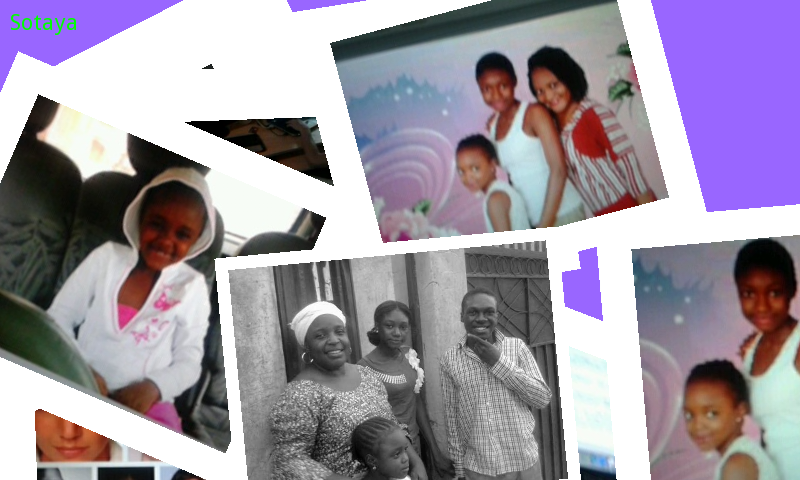
\includegraphics[width=100mm]{viewer.png}
\caption{Scatter images in Viewer}
\label{overflow}
\end{figure}    

The "imagesApp" that was created needs to  call the method {\it run()}, which tells kivy that everything is set and we are ready to show the user the result. Note that this is just the backend code, the code for the design needs to also be implemented in order to be able to view the images. The first class in the listings "Frame" is a kiyy feature that lets the images be scattered on the screen.

\section{Eye Droid Activities}
This project contains four activities, i.e four user interfaces.

\subsection{Main Activity}
The {\bf main activity} in this project which can otherwise be refereed to as the "menu", contains image buttons that can be used to navigate from one activity to the other, this navigation is achieved by the use of intents.

\begin{lstlisting}[label=main-oncreate,caption=Implementation of main activity onCreate method] 
@Override
protected void onCreate(Bundle savedInstanceState) {
	super.onCreate(savedInstanceState);
	setContentView(R.layout.activity_list_item);

	preview = (ImageButton) findViewById(R.id.imageButton1);
	...
	viewer = (ImageButton) findViewById(R.id.imageButton4);

	preview.setOnClickListener(new OnClickListener() {

		@Override
		public void onClick(View v) {
			startPreviewActivity();
		}
	});

	...

	});

	viewer.setOnClickListener(new OnClickListener() {

		@Override
		public void onClick(View v) {
			PackageManager pm = getPackageManager();
			Intent appStartIntent = pm	.getLaunchIntentForPackage("org.plaix.viewer");
			try{
				startActivity(appStartIntent);
			}catch(Exception x){
				Log.d("MainActivity", "Application not Found: "+x.getMessage());
				Toast.makeText(getApplicationContext(), "Module not installed", Toast.LENGTH_SHORT).show();
			}

		}
	});

}
\end{lstlisting} 

In the main activity, four image buttons objects were instantiated in the {\it onCreate()} method. The views were initialized by calling the {\it findViewById()} method (which receives an id of the particular view as parameter) on the object. An {\it onClickListener} event is then set on each of the buttons so that when they are clicked, the methods implemented to start each of the activities are executed, the methods are {\it startPreviewActivity(), startReviewActivity(), startSettingsActivity()}.

As for the Viewer module which is an application level module, it is located on the same device (if installed) and starting it involves setting the same {\it onClickListener()} on the button but with a slightly different implementation. To start an application outside the current application, a package manager object is created and instantiated by calling the {\it getPackageManager()} method, a new intent is also created by calling the {\it getLaunchIntentForPackage()} which takes in a parameter being the application's package name as installed on the device. After which the application is finally started by the use of the {\it startActivity()} method passing it the instantiated intent.

\begin{lstlisting}[label=activity-starter,caption=Activity starter] 
public void startPreviewActivity() {
	startActivity(new Intent(this, PreviewActivity.class));
}     
\end{lstlisting} 

The code responsible for starting the three activities situated in the same application is shown in listing 6.12. Each take the same format, the {\it startActivity()} method is called by passing it an intent as a parameter, within the intent, the context of the application and the activity's class needs to be supplied to the intent.

\begin{lstlisting}[label=back-button-press,caption=Returning to previous event when back button is pressed] 
@Override
public void onBackPressed() {

	AlertDialog.Builder alertbox = new AlertDialog.Builder(this);
	alertbox.setTitle("Warining!");
	alertbox.setMessage("Are you sure you want to exit?");

	alertbox.setPositiveButton("Yes",
			new DialogInterface.OnClickListener() {
				public void onClick(DialogInterface arg0, int arg1) {
					onDestroy();
					Intent intent = new Intent(Intent.ACTION_MAIN);
					intent.addCategory(Intent.CATEGORY_HOME);
					intent.setFlags(Intent.FLAG_ACTIVITY_NEW_TASK);
					startActivity(intent);
					finish();
				}
			});

	alertbox.setNegativeButton("No", new DialogInterface.OnClickListener() {
		public void onClick(DialogInterface arg0, int arg1) {
		}
	});

	alertbox.show();

}
\end{lstlisting}

When back button is pressed, it needs to be controlled, listing 6.13 shows the implementation of the back button press event handler, which creates a dialogue box with two option buttons "yes", "no" and a warning message that ask the user if he/she wants to really exit the application. This was developed to make the application more user friendly and to control the accidental press of the back button. Within the code snippet, it is seen that the application is being finished by calling the {\it finish()} method, this ends the activity's processes and destroys it.

\begin{figure}[ht!]
\centering
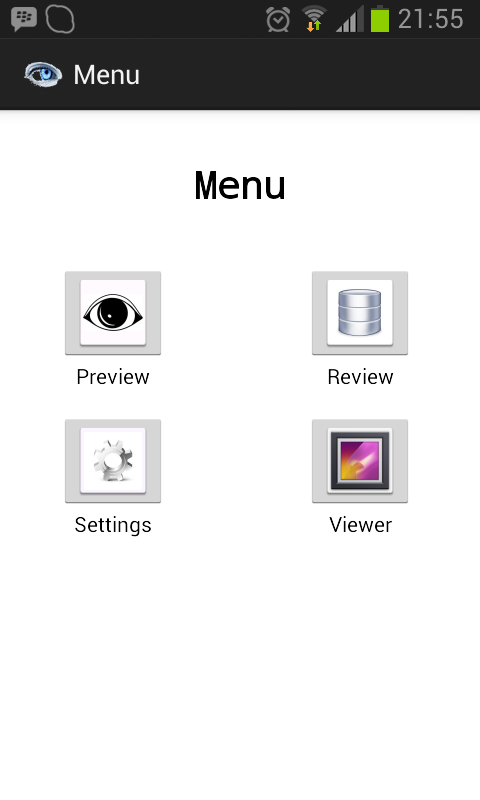
\includegraphics[width=70mm]{main.png}
\caption{Layout of Main Activity}
\label{overflow}
\end{figure}    


\subsection{Preview Activity}
The {\bf preview activity} can be regarded as the main part of this project since most of the main functionalities of the application exist here and it took 70 percent of the whole development time. This activity implements the {\bf camera preview} and sets a face detection event on each of the preview frames generated. This allows the actual real time detection, notification and logging of the events happening within this activity.

\begin{lstlisting}[label=preview-oncreate,caption=Implementation of the preview activity onCreate method] 
@Override
protected void onCreate(Bundle savedInstanceState) {
	super.onCreate(savedInstanceState);
	setContentView(R.layout.preview);

	msg = "Preview started";
	sendMsg(msg, "start");

	surfaceView = (SurfaceView) findViewById(R.id.surfaceView);
	surfaceHolder = surfaceView.getHolder();
	surfaceHolder.addCallback(this);
	surfaceHolder.setType(SurfaceHolder.SURFACE_TYPE_PUSH_BUFFERS);
	capture = (Button) findViewById(R.id.button1);
	face = (TextView) findViewById(R.id.textView1);
		
	getWindow().setFlags(WindowManager.LayoutParams.FLAG_KEEP_SCREEN_ON,
			WindowManager.LayoutParams.FLAG_KEEP_SCREEN_ON);
} 
\end{lstlisting}

The {\it onCreate()} method as discussed under activity life cycle of android application is the first method that is called when an activity is started. The implementation of the {\it onCreate()} method of the preview activity shows the instantiation of several objects, amongst which are the {\it surfaceView} and the {\it surfaceHolder} which is the surface in which the view is placed on. A callback event handler was set to the {\it surfaceHolder} on the given context so that whenever a preview frame is drawn, an implementation method of the {\it SurfaceHolder.Callback} will be executed. The surface holder type has to be set to  "SURFACE\_TYPE\_PUSH\_BUFFERS" which generates several buffers for the surface view.

For the implementation of a {\bf SurfaceHolder.Callback} implementation, there are three important methods that needs to be overridden and implemented. {\it surfaceCreated()} which is called immediately after the surface is created, {\it surfaceChanged()} is called immediately after any structural changes (format or size) have been made to the surface and {\it surfaceDestroyed()} This is called immediately before a surface is being destroyed.

\begin{lstlisting}[label=surface-created,caption=Implementation of surfaceCreated method] 
@Override
public void surfaceCreated(SurfaceHolder holder) {
	camera = Camera.open();
	if (camera != null) {
		try {
			camera.setPreviewDisplay(holder);
		} catch (Exception x) {
			camera.release();
			camera = null;
			Log.d(PreviewActivity.class.getName(),
				"Error in surface created: [" + x.getMessage() + "]");
		}
	} else
		Log.d(PreviewActivity.class.getName(), "Camera null");
}
\end{lstlisting}

Inside the surface created method, the camera instance that was created needs to be initialized (i.e opened) by calling the {\it Camera.open()} method on it and the preview display of the camera needs to be set to the surface holder that was earlier created.
\begin{lstlisting}[label=surface-changed,caption=Implementation of surfaceChanged method] 
@Override
public void surfaceChanged(SurfaceHolder holder, int format, int width,
		int height) {

	if (surfaceHolder.getSurface() == null) {
		Log.d(activityName(), "SurfaceHolder is null");
		return;
	}

	if (camera != null && !inPreview) {
		Camera.Parameters parameters = camera.getParameters();
		Camera.Size size = getPreviewSize(width, height, parameters);

		if (size != null) {
			parameters.setPreviewSize(size.width, size.height);
			camera.setParameters(parameters);
			camera.setDisplayOrientation(0);
			camera.startPreview();
			infBitmap = Bitmap.createBitmap(size.width, size.height,
					Bitmap.Config.RGB_565);
				
			inPreview = true;
			int buffSize = size.width * size.height
					* ImageFormat.getBitsPerPixel(parameters
					.getPreviewFormat()) / 8;
			byte[] Buffer = new byte[buffSize];
			camera.setPreviewCallbackWithBuffer(this);
			camera.addCallbackBuffer(Buffer);
		}

	} else
		Log.d(activityName(), "Camera null");
}  

private Camera.Size getPreviewSize(int width, int height,
			Camera.Parameters parameters) {
		Camera.Size result = null;

		for (Camera.Size size : parameters.getSupportedPreviewSizes()) {
			if (size.width <= width && size.height <= height) {
				if (result == null) {
					result = size;
				} else {
					int resultArea = result.width * result.height;
					int newArea = size.width * size.height;

					if (newArea > resultArea) {
						result = size;
					}
				}
			}
		}
		return result;
	} 
}
\end{lstlisting}	

After setting up the camera environment and display holder in the {\it surfaceCreated()} method, the next method that is on the line is the {\it surfaceChanged()} method. Within this, one has to always check if the surface holder is "null" or not, same goes to the camera instance. The parameters of the camera needs to be set by finding the best preview size possible using the {\it getPreviewSize()} method, this method goes through all the supported preview sizes checking which of the supported sizes is approximately equal to the one generated by the camera. This size's width and height is set to the parameter instance of the camera along side other configurations such as the orientation of the camera. When the camera is configured, the preview is started by calling the {\it camera.startPreview()} method. 

In the {\it surfaceChanged()} method, the buffer size of a preview frame is gotten by first creating a bitmap image with the size (width and height) of the camera preview and using a formula with the appropriate variables to calculate an approximate buffer size, the preview callback with buffer is set to this context and the buffer size is passed to the {\it camera.addCallbackBuffer()} method. This allows the method {onPreviewFrame()} method to be called and enabled to use the buffer size in generating preview frames.

\begin{lstlisting}[label=onPreview-frame,caption=Method for generating preview frames]
public void onPreviewFrame(byte[] data, Camera camera) {

	YuvImage image = new YuvImage(data, ImageFormat.NV21,
	    infBitmap.getWidth(), infBitmap.getHeight(), null);

	Rect rectangle = new Rect();
	rectangle.bottom = infBitmap.getHeight();
	rectangle.top = 0;
	rectangle.left = 0;
	rectangle.right = infBitmap.getWidth();
		
	ByteArrayOutputStream outStream;
	outStream = new ByteArrayOutputStream();
	
	stat = image.compressToJpeg(rectangle, 100, outStream);
	
	detector = new FaceDetector(infBitmap.getWidth(),
			infBitmap.getHeight(), NUM_FACES);

	BitmapFactory.Options inf = new BitmapFactory.Options();
	inf.inPreferredConfig = Bitmap.Config.RGB_565;
	bitImage = BitmapFactory.decodeStream(
	new ByteArrayInputStream(outStream.toByteArray()), null, inf);
		
	Arrays.fill(faces, null);
	facesDetected = detector.findFaces(bitImage, faces);
		
	SharedPreferences sPref;
	sPref = getSharedPreferences(PREF_NAME, 0);
		
	if(sPref.getInt("delay", 0) != 0)
		delay = sPref.getInt("delay", 30) * nanoSec;
		
	if (facesDetected > 0) {
		if (getCurrentTime() - lastTimeStamp >= delay) {
		   msg = facesDetected + " Face Detected";
		   sendMsg(msg, "face");
		   output.saveFace(bitImage);

		   email = sPref.getString("email", "nil");
		   password = sPref.getString("password", "nil");
		   phoneNumber = sPref.getString("phone", "nil");

		   if (sPref.getBoolean("emailCheck", false)) {
		      if (email == "nil" || password == "nil") {
		 	Toast.makeText(getApplicationContext(),
			"Email Settings not set ", Toast.LENGTH_SHORT)
				.show();
		       } else {
			   new Thread() {
				public void run() {
				    sendMail(email, password, output.getPath());
				}
			   }.start();
		       }
		    }

		   if (sPref.getBoolean("phoneCheck", false)) {
                          if (phoneNumber == "nil") {
		         	Toast.makeText(getApplicationContext(),
			"Phone Settings not set", Toast.LENGTH_LONG)
			.show();
		        } else {
		          	message = "Theres an intruder in your house.";
				sendSms(phoneNumber, message);
                          }
		    } else {
			Toast.makeText(getApplicationContext(),
			"Phone Settings not checked", Toast.LENGTH_LONG)
			.show();
                      }
		   lastTimeStamp = getCurrentTime();
	     }
			
	    switch (facesDetected) {
		case 1:
			face.setText(facesDetected + " Face detected");
			break;
		default:
			face.setText(facesDetected + " Faces detected");
	     }

	} else
		face.setText("No face found");

	capture.setOnClickListener(new OnClickListener() {
              @Override
	      public void onClick(View v) {
		output.saveFrame(bitImage);
		msg = "Image captured";
		sendMsg(msg, "capture");
		Toast.makeText(getApplicationContext(), "Image Captured",
				Toast.LENGTH_SHORT).show();
	      }
	});

	camera.addCallbackBuffer(data);
}
\end{lstlisting}

Listing 6.17 shows the implementation of the {\it onPreviewFrame()} method which is called whenever a preview frame is generated providing the frame as  {\it byte[]} data. This data is then converted to a YUVImage of format NV21, a rectangle is created with the size information gotten from {\it infBitmap} created in the {\it surfaceChanged()} method, a {\it ByteArrayOutputStream} instance is created and then the YUVImage is compressed as JPEG image into the outpuStream using the rectangle object that was created. With this output stream, a bitmap image is created using {\it BitmapFactory.decodeStream()} method passing the out stream which is converted to a byte array.

A {\it FaceDetector} object that was created is instantiated using the "infBitmap" information and setting the max number of faces as suited. A {\it FaceDetector.Face[]} array is then cloned using {\it Arrays.Fill()} method and initializing it to null, then faces are detected by calling {\it detector.findFaces()} passing it the parameters "bitImage" which is the bitmap image created from the data[] and "faces" which is the {\it FaceDetector.Faces[]} clone that was created, this method goes through the bitmap image, find the faces (which number is less than or equal to the maximum number of faces provided) and fill them into the faces array. 

The code that follows shows the retrieval of "email", "password" and "phone number" from shared preferences with the truth value of whether the check boxes of both email and phone notification is check, if they are, the system automatically notifies the user by both mediums using the notification module. If the value of those variables are null, that means they have not been set, the user is then notified via splash display. on click event is set on the capture button, when it is clicked, the activity uses the input output module to save the frame on the device storage drive.

\begin{lstlisting}[label=send-intent,caption=Medium to which preview activity sends messages to Logger Module]
public void sendMsg(String msg, String key) {
	Intent sendIntent = new Intent();
	sendIntent.setClass(this, LoggerService.class);
	sendIntent.putExtra(key, msg);
	startService(sendIntent);
}
\end{lstlisting} 	

The implementation of one of the ways modules communicate is by the use of {\bf intents}, listings 6.18 shows the creation of an intent, and the way message is bundled into it as "EXTRAS" and sent as a call to the method {\it startService()}.

\begin{figure}[ht!]
\centering
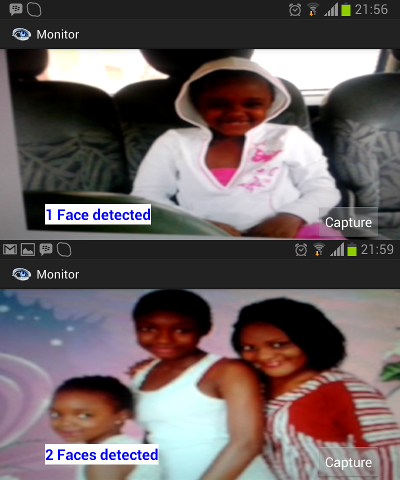
\includegraphics[width=90mm]{preview.png}
\caption{Face detection, Preview Activity}
\label{overflow}
\end{figure}    
\newpage
\subsection{Review Activity}
{\bf Review activity} is tasked with retrieving all the contents of the log(database), formatting and displaying it to the user. This activity makes use of the database module and notifier module. 

\begin{lstlisting}[label=review-oncreate,caption=Implementation of review activity onCreate() method]
@Override
protected void onCreate(Bundle savedInstanceState) {
    super.onCreate(savedInstanceState);
    setContentView(R.layout.activity_review);        
    logRecord = (TextView) findViewById(R.id.textView1);
        
    LogHelper helper = new LogHelper(this);
    log = helper.getAllEvents();
        
    sb = new StringBuilder();
    for(LogModel mod : log){
        	sb.append(mod.toString()).append("\n");
    }        
    logRecord.setText(sb.toString());
}
\end{lstlisting}

As it is for any other activity, {\it review activity} has to implement the {\it onCreate()} method. Within this method, database module is imported and an instance of "LogHelper" is created, with this log helper, the {\it LogHelper.getAllEvents()} method is called on an array list and this data in the array list is formatted by using the java "StringBuilder" after which the text is set to the display view.

The activity also provides the possibility for the user to wipe the database and to upload the log file via email using the notifier module where the java mail is implemented.

\begin{figure}[ht!]
\centering
\includegraphics[width=60mm]{Review.png}
\caption{Layout of Review Activity}
\label{overflow}
\end{figure}    

\subsection{Settings Activity}
The settings activity's task is trivial yet important. From this activity, the user information can be set and stored in the shared preferences so that other activities such as the preview and review activities can access the data and use them when notifying or uploading.

\begin{lstlisting}[label=settings-save,caption=Implementation of the settings "save" option menu]
@Override
public boolean onCreateOptionsMenu(Menu menu) {
    menu.add("Save").setOnMenuItemClickListener(
	new OnMenuItemClickListener() {

              @Override
	     public boolean onMenuItemClick(MenuItem item) {
          	SharedPreferences userData = getSharedPreferences(
			PREF_NAME, 0);

		Editor editor = userData.edit();
		editor.putString("email", email.getText().toString());
		editor.putString("password", password.getText()
				.toString());
		editor.putString("phone", phoneNo.getText().toString());
		editor.putBoolean("emailCheck", emailNotifier.isChecked());
		editor.putBoolean("phoneCheck", phoneNotifier.isChecked());
		editor.putInt("delay", Integer.parseInt(delay.getText().toString()));
		editor.commit();
		Toast.makeText(getApplicationContext(), "Data Saved",
				Toast.LENGTH_SHORT).show();
		finish();						
		return true;
	    }
         });
     return true;
}

\end{lstlisting}

The important method in the settings class worth discussing is the {\it onCreateOptionsMenu()} method. This method is mainly for creating options menu that appear when one presses the menu button on an android device, event handlers can be set to this menus and are executed when clicked on. The menu here is the "save" menu, when this menu is clicked, the values put into the entry fields are retrieved, a shared preference instance is initialized with the preference name and a space is made on the device. Each of the value retrieved from the entry fields is written into this shared preference space as a "key" and "value" pair using an "Editor" instance which writes them with the {\it Editor.put"Type"()} method, where Type can be string, integer, float e.t.c depending on the type of value. Returning true enables the use of options menu.

\begin{figure}[ht!]
\centering
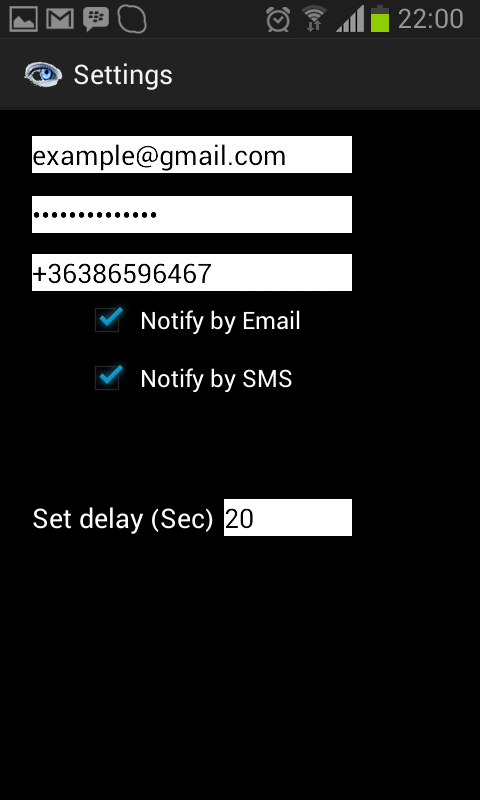
\includegraphics[width=60mm]{settings.png}
\caption{Layout of Settings Activity}
\label{overflow}
\end{figure}    
 

\chapter{Conclusion}
In this thesis, I researched on modular development approach and provided information on the concept. The approach provides a solution to the problem of developing large systems either in teams or as an individual. Following the approach, there are two important development phases which I took on. 

{\bf Modular development} as discussed is nothing more than a development approach that lays its basis on separation of concerns, it encourages the idea of dividing a system into smaller functional modules, developing those modules independent of others and leaving no dependency between two modules unless a module needs another to achieve its goal. This approach also puts emphasis on design first, {\bf modular design}, then implementation, {\bf modular programming}.

Designing a system before implementation is mandatory in this development approach, so i provided the structure of the system, an architectural diagram and two UML models of the system which was used in the implementation phase. This models are the {\bf Use Case diagram} which shows the different use case i.e ways users interact with the system and a {\bf Class Diagram} which shows the different classes of the system and the relationship between them.

The {\bf eye droid} system is an android application which was developed for android devices with the aid of the android development kit. The languages used to implement this system are the Java  programming language which is android's native programming language and Python programming language (Kivy's back-end language). Kivy is an open source development framework which enables rapid application development and can be compiled for multiple platforms.    

The application system is a surveillance system which allows users to use their android devices to monitor a particular environment. This application utilizes the android camera component to detect faces and notifies the user via both SMS and EMAIL in real time. Also the application keeps a log of the events that happened during the camera preview and saves the faces that where detected on the device's storage. The log can be reviewed by the user with the review activity and the faces can be viewed using the viewer module.

From this thesis, I can deduce that it is much more easier and flexible to develop complex software systems by using modular development approach and this concept can be used in android development. I used the feature of packages provided by Java  to package modules and this modules can be compiled individually as .jar files and imported to any project that its needed. This is not the only type of modules, complete android applications themselves can be modules, and can be integrated into a software system by the use of intents, illustration of that is the viewer module which i developed as an individual application and the way its integrated can be seen in the main activity.

There is a lot of extension that can be done to this application, in the future, i intend to extend this system to provide the support for motion detection, face tracking and go to the extent of developing an easier way modules can be integrated into android system. I also intend on researching and experimenting different ways modularity can be achieved in various platforms.



 \chapter{Bibliography}
\begin{enumerate}

\item J�rgen Haas.  Modular programming.\\
{\it http://www.about.com/}
  
\item Seif Haridi; Nils Franz�n.7. Modules and Interfaces (Mozart Documentation) \\
{\it http://www.mozart-oz.org/documentation/index.html}
  
\item Clark, K.B. and Baldwin, C.Y. Design Rules. Vol. 1: The Power of Modularity.\\ 
Cambridge, Massachusetts: MIT Press 2000 ISBN 0-262-02466-7

\item Modular Programming\\
{\it http://www.eng.fsu.edu/~dommelen/courses/cpm/notes/progreq/node2.html}

\item Modular Programming\\
{\it http://c2.com/cgi/wiki?ModularProgramming}

\item Technopedia: Modular Programming\\
{\it http://www.techopedia.com/definition/25972/modular-programming}

\item Sun Microsystems, (2007) Benefits of Modular Programming\\
{\it https://netbeans.org/project\_downloads/usersguide/rcp-book-ch2.pdf}

\item Bernaridho I Hutabarat, Ketut E. Purnama, Mochammad Hariadi: Module, Modular Programming, and Module-Based Encapsulation : Critiques and Solution
  
\item James Gosling, Bill Joy, Guy Steele, Gilad Brachan (2005) The Java Language Specification
Third Edition ISBN 0-321-24678-0.

\item Martin Fowler, UML Distilled: A Brief Guide to the Standard Object Modeling\- Language (3rd Edition), 
Addison-Wesley Professional

\item UML Standard Diagrams: Tutorials Point \\
{\it http://www.tutorialspoint.com/uml/} 

\item Cay S. Horstmann, (2002) UML Diagrams\\
{\it http://www.cs.sjsu.edu/~drobot/cs146/UMLDiagrams.htm}

\item Marc Hamilton (1999) Software Development: A Guide to Building Reliable Systems p.48

\item Android Code Analysis\\
{\it http://www.ohloh.net/p/android}

\item Android OS Statistics\\
{\it http://www.idc.com/getdoc.jsp?containerId=prUS23946013}

\item Concepts of Android OS components\\
{\it http://www.android\-app\-market.com/android\-architecture.html}

\item Application Statistics \\
{\it http://www.appbrain.com}

\item ELinux: Android Architecture\\
{\it http://elinux.org/Android\_Architecture}

\item Kivy: Kivy Architecture\\
{\it http://kivy.org/docs/guide/architecture.html}

\item Oracle: Java Standard Edition API\\
{\it http://docs.oracle.com/javase/6/docs/api/}  

\item Android Activity Lifecycle
{\it http://www.android-app-market.com/android-activity-lifecycle.html}

\item Android API Guide\\
{\it http://developer.android.com/guide/components/index.html}

\item Android API References\\
{\it http://developer.android.com/reference/packages.html}

\item Android Development Tools: Setting up Android Development Environment\\
{\it http://developer.android.com/tools/index.html}

\item Lars Vogel: Android Intents
{\it http://www.vogella.com/articles/AndroidIntent/article.html}

\item Sample implementations for Android Developers\\
{\it http://developer.android.com/samples/index.html}

\item Kivy Framework Documentation\\
{\it http://kivy.org/docs/}

\item Python Standard Documentation\\
{\it http://www.python.org/doc/}
    
\end{enumerate}    
\end{document}